\documentclass[a4paper]{article}

\usepackage{amsmath}
\usepackage{hyperref}
\usepackage{biblatex}
\usepackage{enumerate}
\usepackage{graphicx}
\usepackage{stmaryrd}
\usepackage[dvipsnames]{xcolor}
\usepackage{listings}
\usepackage{float}
\addbibresource{refs.bib}

\begin{document}

\author{
  Sebastian Miles \\
  \href{mailto:miless@chalmers.se}{miless@chalmers.se}
  \and
  Olle Lapidus \\
  \href{mailto:ollelap@chalmers.se}{ollelap@chalmers.se}
}
\title{DAT565/DIT407 Assignment 6}
\date{2024-10-11}

\maketitle
\section*{Problem 1}
We verify that the images are 28x28 pixels grayscales and plot a few of the images.
\begin{figure}[H]
	\begin{center}
		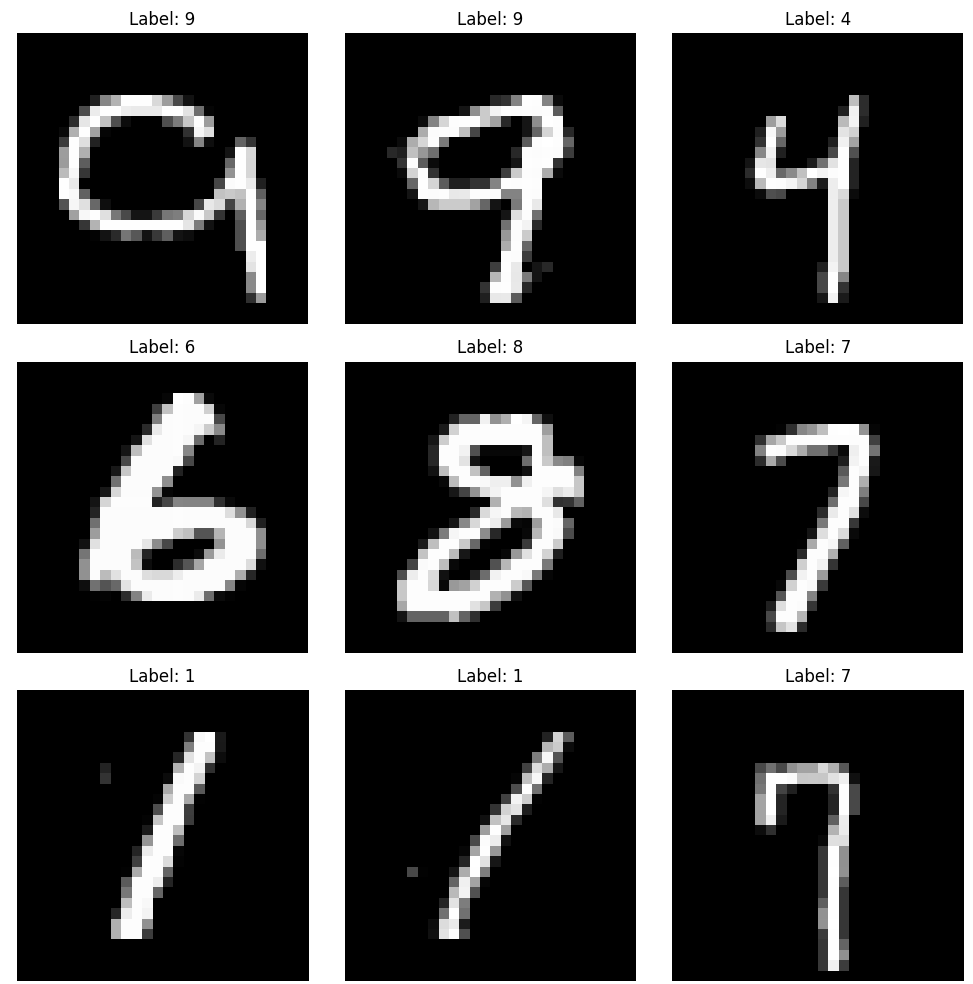
\includegraphics[scale=0.4]{datasets.png}
		\caption{Various images from the datasets}
		\label{hist}
	\end{center}
\end{figure}

\section*{Problem 2}
We train the data with a single hidden layer. We put the hidden layer size as 128 and the learning rate for SGD as 0.01. The accuracy over 10 epochs is shown in table \ref{tab}.
\begin{table}[H]
	\centering
	
	\begin{tabular}{|c|c|}
		\hline
		Epoch & Accuracy \\
		\hline
		1 & 79.45\% \\
		\hline
		2 & 82.06\% \\
		\hline
		3 &  84.35\%\\
		\hline
		4 &  83.96\%\\
		\hline
		5 &  84.61\%\\
		\hline
		6 &  85.36\%\\
		\hline
		7 &  84.10\%\\
		\hline
		8 &  85.57\%\\
		\hline
		9 &  84.92\%\\
		\hline
		10 &  86.75\%\\
		\hline
	\end{tabular}
	\caption{Accuracy of the test data over 10 epochs. }
	\label{tab}
\end{table}

\section*{Problem 3}
For this problem we used $\text{weight decay}  = 0.0001$ and
$\text{learning rate} = 0.04$. The accuracies are displayed in table \ref{tab2}. The accuracy seems to plateau at around 98\%, which is also what we were supposed to reach.

\begin{table}[H]
	\centering
	\begin{tabular}{|c|c|}
		\hline
		Epoch & Accuracy \\
		\hline
		1 & 90.61\% \\
		\hline
		2 & 94.65\%\\
		\hline 
		3 & 94.68\%\\
		\hline 
		4 & 95.81\%\\
		\hline 
		5 & 96.90\%\\
		\hline 
		6 & 94.19\%\\
		\hline 
		7 & 97.10\%\\
		\hline 
		8 & 97.29\%\\
		\hline 
		9 & 97.29\%\\
		\hline 
		10 & 97.19\%\\
		\hline 
		11 & 97.85\%\\
		\hline 
		12 & 97.76\%\\
		\hline 
		13 & 98.05\%\\
		\hline 
		14 & 97.92\%\\
		\hline 
		15 & 97.90\%\\
		\hline 
		16 & 97.21\%\\
		\hline 
		17 & 98.04\%\\
		\hline 
        18 & 98.12\%\\
		\hline 19 & 98.10\%\\
		\hline 20 & 98.07\%\\
		\hline 21 & 98.13\%\\
		\hline 22 & 98.02\%\\
		\hline 23 & 98.11\%\\
		\hline 24 & 97.80\%\\
		\hline 25 & 98.20\%\\
		\hline 26 & 98.23\%\\
		\hline 27 & 98.17\%\\
		\hline 28 & 98.21\%\\
		\hline 29 & 98.22\%\\
		\hline 30 & 98.24\%\\
		\hline 31 & 98.29\%\\
		\hline 32 & 98.22\%\\
		\hline 33 & 98.22\%\\
		\hline 34 & 98.28\%\\
		\hline 35 & 98.30\%\\
		\hline 36 & 98.30\%\\
		\hline 
		37 & 98.30\%\\
		\hline 
		38 & 98.36\%\\
		\hline 
		39 & 98.28\%\\
		\hline 
		40 & 98.34\%\\
		\hline
	\end{tabular}
	\caption{Accuracy of the test data over 40 epochs with two hidden layers. }
	\label{tab2}
\end{table}
\section*{Problem 4}
In this model we first have a convolution layer with 32 filters and 3x3 kernel, and max pooling with a 2x2 window.
In the second layer we have 64 filters with a 3x3 kernel and a 2x2 max pooling. Finally we have a hidden layer with 128 neurons. In between every layer we use ReLU activation which adds non-linearity to the model. We also used the same weight decay and learning rate as in problem 3. The accuracy for 40 epochs is shown in table \ref{tab3}. We note that the accuracies plateau at around $99.1\%$ meaning that we have likely reached the best accuracy for the model, and running it for more epochs would be a waste.
\begin{table}[H]
	\centering
	\begin{tabular}{|c|c|}
	\hline
	Epoch & Accuracy \\
	\hline1 & 97.34\% \\
	\hline2 & 98.16\% \\
	\hline3 & 98.50\% \\
	\hline4 & 98.29\% \\
	\hline5 & 98.80\% \\
	\hline6 & 98.61\% \\
	\hline7 & 98.88\% \\
	\hline8 & 97.84\% \\
	\hline9 & 98.76\% \\
	\hline10 & 99.08\%\\
	\hline11 & 99.17\%\\
	\hline12 & 99.12\%\\
	\hline13 & 99.04\%\\
	\hline\vdots & \vdots\\
	\hline37 & 99.10\%\\
	\hline38 & 99.11\%\\
	\hline39 & 99.11\%\\
	\hline40 & 99.15\%\\
	\hline\end{tabular}
	\caption{Accuracy of the test data over 40 epochs with a convolution NN. }
	\label{tab3}
\end{table}

\printbibliography
\appendix

\section*{Code}
\label{app:excode}

\lstset{
	language=Python,
	basicstyle=\ttfamily,
	commentstyle=\color{OliveGreen},
	keywordstyle=\bfseries\color{Magenta},
	stringstyle=\color{YellowOrange},
	numbers=left,
	frame=tblr,
	breaklines=true,
	postbreak=\mbox{\textcolor{red}{$\hookrightarrow$}\space},
}
\begin{lstlisting}
import torch
import torch.nn as nn
import torch.optim as optim
import torchvision.transforms as transforms
import torchvision.datasets as datasets
from torch.utils.data import DataLoader

input_size = 28 * 28
hidden_size = 128
output_size = 10
weight_decay = 0.0001
learning_rate = 0.04

transform = transforms.Compose([
    transforms.ToTensor(),
    transforms.Normalize((0.5,), (0.5,))  # Normalize to [-1, 1]
])

train_dataset = datasets.MNIST(root='./mnist_data', train=True, download=True, transform=transform)
test_dataset = datasets.MNIST(root='./mnist_data', train=False, download=True, transform=transform)

train_loader = DataLoader(train_dataset, batch_size=64, shuffle=True)
test_loader = DataLoader(test_dataset, batch_size=64, shuffle=False)


def train_model(model, train_loader, test_loader, num_epochs):
    criterion = nn.CrossEntropyLoss()
    optimizer = optim.SGD(model.parameters(), lr=learning_rate, weight_decay=weight_decay)

    for epoch in range(1, num_epochs + 1):
        model.train()
        for batch_idx, (data, target) in enumerate(train_loader):
            optimizer.zero_grad()
            #output = model(data.view(-1, 28*28))  # Cant do this with model3
            output = model(data)
            loss = criterion(output, target)
            loss.backward()
            optimizer.step()
        
        test_loss, accuracy = validate(model, test_loader, criterion)
        print(f'{epoch} & {accuracy:.2f}\\%')
    
    return model

def validate(model, test_loader, criterion):
    model.eval()
    test_loss = 0
    correct = 0
    with torch.no_grad(): # disable gradient calculation for validation
        for data, target in test_loader:
            #output = model(data.view(-1, 28*28)) # Cant do this with model3
            output = model(data)
            test_loss += criterion(output, target).item()
            pred = output.argmax(dim=1, keepdim=True) 
            correct += pred.eq(target.view_as(pred)).sum().item()

    test_loss /= len(test_loader.dataset)
    accuracy = 100.0 * correct / len(test_loader.dataset)
    return test_loss, accuracy


model1 = nn.Sequential(
    nn.Linear(28*28, hidden_size),
    nn.ReLU(),
    nn.Linear(hidden_size, output_size)
)


#train_model(model1, train_loader, test_loader, num_epochs=10)

model2 = nn.Sequential(
    nn.Linear(28*28, 500),
    nn.ReLU(),
    nn.Linear(500, 300),
    nn.ReLU(),
    nn.Linear(300, 10),
)

#train_model(model2, train_loader, test_loader, num_epochs=40)

model3 = nn.Sequential(
    nn.Conv2d(in_channels=1, out_channels=32, kernel_size=3, stride=1, padding=1),
    nn.ReLU(),
    nn.MaxPool2d(kernel_size=2, stride=2),

    nn.Conv2d(in_channels=32, out_channels=64, kernel_size=3, stride=1, padding=1),
    nn.ReLU(),
    nn.MaxPool2d(kernel_size=2, stride=2),

    nn.Flatten(),
    nn.Linear(64 * 7 * 7, 128),
    nn.ReLU(),

    nn.Linear(128, 10)
)

train_model(model3, train_loader, test_loader, num_epochs=40)
\end{lstlisting}

\end{document}
